% Latex课程报告模板 袁老师封面版
 
\documentclass{article}
\usepackage[UTF8,zihao=-4]{ctex}
\usepackage{amsfonts} 
\usepackage{amsmath} 
\usepackage[top=2.54cm, bottom=2.54cm, left=3.18cm, right=3.18cm]{geometry}
\geometry{paper=a4paper}
\usepackage{graphicx}
\usepackage{gbt7714}
\usepackage{setspace}
\usepackage{indentfirst}
\usepackage{titlesec}
\usepackage{fancyhdr}  
\usepackage{listings} % 引入 listings 宏包
\usepackage{xcolor}   % 支持颜色  



%%%%%%%%%%%%% 自定义设定 %%%%%%%%%%%%


% 自定义字体
\newCJKfontfamily\heititext{SimHei}[
  Path = C:/Windows/Fonts/,  % Windows字体目录
  AutoFakeBold = 2,        % 加粗强度(3.5为最佳视觉效果)
]


\newCJKfontfamily\simsuntext{SimSun}[
  Path = C:/Windows/Fonts/,  % Windows字体目录
  AutoFakeBold = 2,        % 加粗强度(3.5为最佳视觉效果)
]

\newCJKfontfamily\hwtext{STXinwei}[
  Path = C:/Windows/Fonts/,  % Windows字体目录
  AutoFakeBold = 2,        % 加粗强度(3.5为最佳视觉效果)
]

% 以下是MacOS自定义字体
% \newCJKfontfamily\heititext{SimHei}[
%   Path = /Users/zhouzhuo/Library/Fonts/,  % Windows字体目录
%   AutoFakeBold = 2,        % 加粗强度(3.5为最佳视觉效果)
% ]

% \newCJKfontfamily\simsuntext{SimSun}[
%   Path = /Users/zhouzhuo/Library/Fonts/,  % Windows字体目录
%   AutoFakeBold = 2,        % 加粗强度(3.5为最佳视觉效果)
% ]

% \newCJKfontfamily\hwtext{simkai}[
%   Path = /Users/zhouzhuo/Library/Fonts/,  % Windows字体目录
%   AutoFakeBold = 2,        % 加粗强度(3.5为最佳视觉效果)
% ]


% 自定义命令
% 三角等号
\newcommand{\triangleq}{\stackrel{\mathrm{def}}{=}} 
% 自定义变量
\newcommand{\TITLE}{文物图纸重建中双目图像处理的单应性的深入理解} %标题
\newcommand{\AUTHOR}{周卓} %作者
\newcommand{\STUDENTNO}{2240201012} %学号
\newcommand{\sizethirty}{\fontsize{30pt}{50pt}}  % 30号字(初号)

% 行距与缩进
\onehalfspacing
\setlength{\parindent}{2em}

% 自定义各级标题格式字体
\titleformat{\section}
  {\heititext \zihao{3} \bfseries \centering}
  {\thesection}
  {1em}{}
\titlespacing{\section}{0pt}{24pt}{18pt}

\titleformat{\subsection}
  {\simsuntext \zihao{4} \bfseries \raggedright}
  {\thesubsection}
  {1em}{}
\titlespacing{\subsection}{0pt}{18pt}{12pt}

\titleformat{\subsubsection}
  {\simsuntext \zihao{-4} \bfseries \raggedright}
  {\thesubsubsection}
  {1em}{}
\titlespacing{\subsubsection}{0pt}{12pt}{6pt}

% 代码块样式定义
\lstset{
    basicstyle=\ttfamily\small, % 基本字体样式
    keywordstyle=\color{blue},  % 关键字颜色
    commentstyle=\color{green}, % 注释颜色
    stringstyle=\color{red},    % 字符串颜色
    numbers=left,               % 显示行号
    numberstyle=\tiny\color{gray}, % 行号样式
    frame=single,               % 边框样式
    breaklines=true,            % 自动换行
    tabsize=4                   % 制表符宽度
}


%%%%%%%%%%%%% 文档开始 %%%%%%%%%%%%

\begin{document}


%%%%%%%%%%%%% 封面页 %%%%%%%%%%%%

\pagestyle{empty}
\begin{flushright}
{
     {\simsuntext \zihao{-4} \bfseries 2024-2025学年第二学期}
    
}
\end{flushright}


\begin{figure}[h]
    \centering
    
\includegraphics[width=0.8\textwidth]{./城院logo3.png}
    % \caption{}
\end{figure}
% \vspace*{12em}
\begin{center}
    {\hwtext\bfseries\sizethirty 
    《现代信号处理技术》\\[1.5\baselineskip]  % 手动调整行距
    课程报告}
\end{center}
\begin{figure}[h]
    \centering
    
\includegraphics[width=0.33\textwidth]{./城院logo2.png}
    % \caption{}
\end{figure}
% \vspace{3em}

\newcommand{\fssi}{\fangsong\zihao{4}}

\begin{center}
{ \fssi % 这里的字号也可以用别的方式修改

\makebox[4em][s]{姓名}:\hspace{1em}\underline{\makebox[14em][c]{\AUTHOR}}\\
\vspace{1em}
\makebox[4em][s]{学号}:\hspace{1em}\underline{\makebox[14em][c]{\STUDENTNO}}\\
\vspace{1em}
\makebox[4em][s]{专业班级}:\hspace{1em}\underline{\makebox[14em][c]{电子信息2402}}\\
\vspace{1em}
\makebox[4em][s]{所在学院}:\hspace{1em}\underline{\makebox[14em][c]{信息与电气工程学院}}\\
\vspace{1em}
\makebox[4em][s]{指导老师}:\hspace{1em}\underline{\makebox[14em][c]{袁建涛}}\\
\vspace{1em}
\makebox[4em][s]{日期}:\hspace{1em}\underline{\makebox[14em][c]{2025.6.17}}\\
}
\end{center}



%%%%%%%%%%%%% 标题 摘要 %%%%%%%%%%%%



\title{\TITLE}
% \author{\AUTHOR~ \STUDENTNO}
\date{}
\maketitle

\thispagestyle{empty}

\begin{center}
  {\heititext\zihao{3}\bfseries 摘要}  % 标题加粗
\end{center}
\vspace{0.5em}
{
    \simsuntext\zihao{-4}\linespread{1.5}\selectfont
    \hspace{2em}图像处理是现代信号处理的重要领域,双目图像处理又是其中的重要课题。本文根据作者的实际项目经历——多视角图像高精度文物图纸重建,深入探讨了平面单应性(Homography)在解决多视角图像透视畸变矫正中的核心作用。从数学上推导了单应矩阵的生成原理,阐释了其连接二维图像与三维空间几何关系和本质。详细阐述了基于匹配点对的单应矩阵估计方法以及关键的归一化处理过程。重点分析了如何从归一化的单应矩阵分解恢复相机旋转运动和带有尺度信息的平移,并指出存在四组数学解及通过正深度约束筛选物理可行解的策略。进一步分析了单应性的典型应用案例:视角旋转校正、共面场景图像拼接、纯旋转运动估计。
    \par  % 确保行距生效
    \vspace{0.5em}
    \noindent{\simsuntext\zihao{-4}\bfseries 关键词:} \simsuntext\zihao{-4}图像处理;单应性;透视校正;运动恢复;
}

%%%%%%%%%%%%% 目录 %%%%%%%%%%%%

\newpage
\pagestyle{plain}
\pagenumbering{roman}
\tableofcontents

%%%%%%%%%%%%% 正文 %%%%%%%%%%%%

\newpage
\pagestyle{fancy}
\fancyhf{}               % 清空默认页眉页脚
\renewcommand{\headrulewidth}{0pt} % 取消页眉线
\pagenumbering{arabic} \setcounter{page}{1} % 重置为阿拉伯数字
\cfoot{第 \thepage\ 页 \hspace{0.5em} 共 \pageref{EndBody} 页}

\section{引言}
\subsection{双目图像处理}

图像处理作为现代信号处理的核心分支,通过算法对图像进行增强、压缩、分析和识别,已成为多学科交叉的关键技术领域。双目图像处理作为该领域的重点课题,通过模拟人类双眼视差原理实现三维感知。双摄像头同步捕获图像,经标定、立体校正和特征匹配(如SIFT/SURF算法)计算视差,生成深度图并重建三维场景。

\subsection{文物图纸重建}
随着文化遗产保护意识的提升与数字技术的迅猛发展,构建高精度文物数字化图纸数据库已成为全球文博领域的核心任务。传统文物记录依赖手工测绘与二维影像,存在效率低、精度受限、信息维度单一等瓶颈。而文物作为不可再生资源,其脆弱性(如彩绘褪色、结构风化)要求记录过程必须非接触、高效率、全息化。在此背景下,融合多视角三维重建与智能图形处理技术的数字化方案,成为实现文物永久性数字存档、虚拟复原与跨学科研究的关键路径,亦是国家“文化数字化战略”的重要实践方向。


文物数字化图纸重建的主流方案采用使用标定板或控制点进行单应性变换(Homography),多视角拍摄-智能透视矫正-参数化线框生成”的全流程解决方案,核心关键问题是:

高精度透视矫正​​:针对非平面文物​(如青铜器曲面、浮雕),设计自适应单应性矩阵估计算法,消除多视角影像的几何畸变。
从矫正影像生成结构化线框图:融合三维点云语义分割与二维矢量生成技术,自动提取拓扑准确的文物轮廓线与结构线,支持CAD格式输出。


文物数字化图纸重建将推动文物档案从“经验型记录”向“数据化孪生”转型,为文物修复提供精准缺损参照、为数字博物馆生成交互式线框模型)、为考古研究的量化形制分析提供核心数据底座,助力文化遗产的精准化保护、系统化传承与智慧化利用。

本文根据作者自己的理解, 对文物图纸重建项目中涉及的平面单应性(Homography)原理,结合计算机视觉理论与文物数字化实践需求,进行的系统性分析推导。全文从数学基础到工程实现逐步展开,重点突出单应性在透视矫正中的核心作用。 

\section{技术基础}

\subsection{单应性介绍}

单应性(Homography)是计算机视觉和射影几何中的核心概念,指两个平面之间的可逆投影映射关系。它能够保持几何体的共线性(直线变换后仍为直线)和交比不变性,广泛应用于图像处理、三维重建等领域。单应性是连接二维图像与三维空间几何关系的关键工具,其矩阵 ${\mathbf{H}}$ 封装了平面间的投影映射规则,是高效解决视觉任务的基础。

\begin{figure}[h]
    \centering
    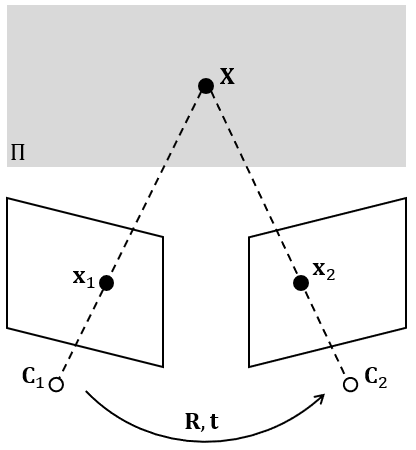
\includegraphics[width=0.5\textwidth]{./xinhaochuli/1.png}
    \caption{当两个摄像机同时看向同一个平面}
    \label{fig:1}
\end{figure}



如图\ref{fig:1}所示\cite{bradski2008learning},设图像坐标系的点$\mathbf{y}_i$ 这里的$\mathbf{y}_i$是齐次坐标,存在矩阵 ${\mathbf{H}}$ 即为单应矩阵,使 $\alpha_g\mathbf{y}_2=\mathbf{Hy}_1$。

\subsection{单应性推导}
    

如图\ref{fig:1}所示,假设有两个相机,光心分别为 ${\mathbf{C}_1}$ 和 ${\mathbf{C}_2}$ ,二者同时拍摄3D空间中的平面 ${\Pi}$ 。
记平面 ${\Pi}$ 上的点为 ${\mathbf{X}} \in \mathbb{R}^3$ ,两个相机之间的相对运动是 $({\mathbf{R}}, {\mathbf{t}})$ 。则该点在两个相机坐标系下的坐标变换为:

\begin{equation} \label{eq:1}  
{\mathbf{X}_2} = {\mathbf{R}}{\mathbf{X}_1} + {\mathbf{t}}
\end{equation}
记平面 ${\Pi}$ 在相机 ${\mathbf{C}_1}$ 坐标系下的参数为 $\{\hat{\mathbf{n}}, d\}$ ,其中 $\hat{\mathbf{n}}$ 是单位平面法向量且背向原点,$d > 0$ 是原点到平面的距离。由于点 ${\mathbf{X}_1}$ 在平面上,因此有
\begin{equation} \label{eq:2}
\hat{\mathbf{n}}^\top{\mathbf{X}_1} = d \Rightarrow \frac{1}{d}\hat{\mathbf{n}}^\top{\mathbf{X}_1} = 1
\end{equation}

将式(\ref{eq:2})直接代入到式(\ref{eq:1}),从而有

$$\begin{aligned}
{\mathbf{X}_2} &= {\mathbf{R}}{\mathbf{X}_1} + {\mathbf{t}}\left(\frac{1}{d}\hat{\mathbf{n}}^\top{\mathbf{X}_1}\right) \\
&= \left({\mathbf{R}} + \frac{1}{d}{\mathbf{t}}\hat{\mathbf{n}}^\top\right){\mathbf{X}_1}
\end{aligned}
$$

矩阵 ${\mathbf{H}} = {\mathbf{R}} + \frac{1}{d}{\mathbf{t}}\hat{\mathbf{n}}^\top$ 即为单应矩阵,它表示从点 ${\mathbf{X}_1}$ 到点 ${\mathbf{X}_2}$ 的线性变换,即 ${\mathbf{X}_2} = {\mathbf{H}}{\mathbf{X}_1}$ 。

将平面$\Pi$上的点投影到各自的归一化平面上,即相机坐标系下$Z=1$的平面。

此时$\lambda _i\mathbf{x} _i= \mathbf{X} _i$, $i= 1, 2$ 。从而更进一步有:

$$\lambda_2\mathbf{x}_2=\lambda_1\mathbf{H}\mathbf{x}_1$$



消除尺度系数,即可得$\mathbf{x}_2\sim\mathbf{H}\mathbf{x}_1$ 。归一化平面上的点$\mathbf{x}_i$可以由图像坐标系的点$\mathbf{y}_i$通过

内参矩阵$\mathbf{K}$获得:

$$\mathbf{K}^{-1}\mathbf{y}_2\sim\mathbf{H}\mathbf{K}^{-1}\mathbf{y}_1\Rightarrow\mathbf{y}_2\sim\mathbf{K}\mathbf{H}\mathbf{K}^{-1}\mathbf{y}_1$$



注意,这里的$\mathbf{y}_i$是齐次坐标。

该式即为更加常见的单应矩阵形式:$\alpha_g\mathbf{y}_2=\mathbf{Hy}_1$ ,即将内参矩阵也包含进单应矩阵中$H\leftarrow \mathrm KHK^{- 1}$。

\subsection{单应矩阵的归一化的推导}

考虑一个估计单应矩阵的情况。图像中应该可以提取出很多的对应点,而四个点且任意三点不共线时,即可估计出一个单应矩阵。使用不同的点对,可能得到一堆单应矩阵的集合$\{\mathbf{H}_{L}^{(1)},\mathbf{H}_{L}^{(2)},\ldots,\mathbf{H}_{L}^{(n)}\}$。

理想情况下,这些单应矩阵还应该是互相成比例的$\lambda^{(1)}\mathbf{H}_{L}^{(1)}=\lambda^{(2)}\mathbf{H}_{L}^{(2)}=\ldots=\lambda^{(n)}\mathbf{H}_{L}^{(n)}$,但本质上描述的是相同的情况。这样的表示很显然是冗余的。

那么有没有一种方法,使得上面的矩阵,通过对自身做某种运算,输出的结果都是相同的呢?解决这个问题的过程就是对单应矩阵做归一化。

单应矩阵的归一化,目标就是找到一个$\mathbf{H}_{L}$,使得对于任意的$\mathbf{H}_{L}^{(i)}$,都能通过归一化操作对应到相同的$\mathbf{H}_{L}$。


形如$\mathbf{H}_{L}=\lambda(\mathbf{R}+\frac{1}{d}\mathbf{t}\hat{\mathbf{n}}^{\top})$的矩阵,其尺度系数$\lambda$被计算为:

$$|\lambda|=\text{med}(\text{svd}(\mathbf{H}_{L}))$$


即$|\lambda|$是$\mathbf{H}_{L}$的第二大的奇异值\cite{ma2004invitation}。

\subsection{单应性矩阵的估计}
给定一组图像坐标系下的匹配点$\{\mathbf{y}_1,\mathbf{y}_2,\ldots,\mathbf{y}_n\}$和$\{\mathbf{y}_1^{\prime},\mathbf{y}_2^{\prime},\ldots,\mathbf{y}_n^{\prime}\}$ ,求出对应的最优单应矩阵$\mathbf{H}$ 。这里假设相机已经预先执行过标定,即内参矩阵$\mathbf{K}$可知。这里将图像坐标系下的像素坐标转换到归一化平面上,即:

$$\mathbf{x}=\mathbf{K}^{-1}\mathbf{y}$$

即可用单应约束$\alpha_g\mathbf{x}=\mathbf{H}\mathbf{x}^{\prime}$ ,根据匹配点对恢复单应矩阵。

将$\alpha_g\mathbf{x}=\mathbf{H}\mathbf{x}^{\prime}$展开:

$$\begin{gathered}\alpha_{g}x_{1}=h_{11}x_1^{\prime}+h_{12}x_2^{\prime}+h_{13}\\\alpha_gx_2=h_{21}x_1^{\prime}+h_{22}x_2^{\prime}+h_{23}\\\alpha_{g}=h_{31}x_1^{\prime}+h_{32}x_2^{\prime}+h_{33}\end{gathered}$$

将第三个式子代入到第一、二个式子消去尺度系数$\alpha_g:$

$$(h_{31}x_1'+h_{32}x_2'+h_{33})x_1=h_{11}x_1'+h_{12}x_2'+h_{13}\\(h_{31}x_1'+h_{32}x_2'+h_{33})x_2=h_{21}x_1'+h_{22}x_2'+h_{23}$$

然后向量化的形式为:
$$\begin{bmatrix}
-x_1' & 0 & x_1'x_1 & -x_2' & 0 & x_2'x_1 & -1 & 0 & x_1 \\
0 & -x_1' & x_1'x_2 & 0 & -x_2' & x_2'x_2 & 0 & -1 & x_2
\end{bmatrix}
\begin{bmatrix}
h_{11} \\
h_{21} \\
h_{31} \\
h_{12} \\
h_{22} \\
h_{32} \\
h_{13} \\
h_{23} \\
h_{33}
\end{bmatrix}
= 0$$

单应矩阵 H 是一个3×3齐次矩阵,但由于尺度等价性(即 H 乘以任意非零常数仍表示同一变换),实际自由度为8。因此,当存在四组匹配点时, 等式左侧将含有八行。此时就可以利用求齐次方程的最小二乘问题来求解:

$$\hat{\mathbf{h}}=\arg\min\|\mathbf{A}\mathbf{h}\|^2,\text{ subject to }\|\mathbf{h}\|^2=1$$

对矩阵 $\mathbf{A}$ 做SVD分解为 $\mathbf{A} = \mathbf{U}\Sigma\mathbf{V}^T$。令$\mathbf{q}=V^T\mathbf{h}$,问题转化为最小化$\|\Sigma\mathbf{q}\|$且$\|\mathbf{h}\|=1$。
$\Sigma$的对角元素降序排列,因此$\mathbf{q}=(0,0,\ldots,1)^T$使目标函数最小。最优解为 $\mathbf{V}$ 的最后一列向量。

注意,由于求解时使用了约束项 $||\mathbf{h}|| = 1$,这个结果和归一化单应矩阵 $\mathbf{H}_L$ 之间差了个尺度系数,执行归一化操作即可。

\subsection{由归一化的单应矩阵恢复相机运动}

给定一个归一化的单应矩阵,形式为$\mathbf{H}=\mathbf{R}+\frac1d\mathbf{t}\hat{\mathbf{n}}^\top$。该矩阵可被分解为$\{\mathbf{R},\frac1d\mathbf{t},\hat{\mathbf{n}}\}$ ,共有四组解,但最多有两种符合物理实际的解\cite{ma2004invitation}。下面推导四组解的配置,并给出如何确定最终的解。
对于任何与平面法线$\hat{\mathbf{n}}$垂直的向量$\mathbf{a}$,$||\mathbf{Ha}||=||\mathbf{Ra}||=||\mathbf{a}||$ ,受到单应矩阵$\mathbf{H}$的作
用后模长保持不变。如果知道了所有与$\hat{\mathbf{n}}$垂直的向量所张成的平面,那么就可以知道$\hat{\mathbf{n}}$ 。对称矩阵$\mathbf{H}^\top\mathbf{H}$的特征值为$\{\alpha_1,\alpha_2,\alpha_3\}$ ,且$\alpha_{2}=1$。对$\mathbf{H}^\top\mathbf{H}$做特征值分解,可得:
$\mathbf{H}^\top\mathbf{H}=\mathbf{V}\Sigma\mathbf{V}^\top$
。其中$\Sigma=\operatorname{diag}(\alpha_1,\alpha_2,\alpha_3)$ , $\mathbf{V}=[\mathbf{v}_1,\mathbf{v}_2,\mathbf{v}_3]\in\mathcal{SO}(3)$ 。这里强制令$\mathbf{V}\in\mathcal{SO}(3)$
。若分解出的$\det(\mathbf{V})<0$ ,则可令$\mathbf{v}_3=-\mathbf{v}_3$,这个特征值分解的结果不变。

对 $\mathbf{v}_3$ 取负的操作,可视作右乘 $\mathbf{V}\begin{bmatrix}1&0&0\\0&1&0\\0&0&-1\end{bmatrix}=\mathbf{VD}=\mathbf{V'}$。

此时 $\mathbf{V'}\mathbf{\Sigma}\mathbf{V'}^\top=\mathbf{VD}\mathbf{\Sigma}D\mathbf{V}^\top=\mathbf{V}\mathbf{\Sigma}\mathbf{V}^\top=\mathbf{H}^\top\mathbf{H}$,即对 $\mathbf{V}$ 的最后一列取负,依然对应着原矩阵。

此时可以将$\mathbf{H}^\top\mathbf{H}=\mathbf{V}\Sigma\mathbf{V}^\top$写成拆分的形式:

$$\begin{cases}\mathbf{H}^\top\mathbf{H}\mathbf{v}_1=\alpha_1\mathbf{v}_1\\\mathbf{H}^\top\mathbf{H}\mathbf{v}_2=\mathbf{v}_2\\\mathbf{H}^\top\mathbf{H}\mathbf{v}_3=\alpha_3\mathbf{v}_3\end{cases}$$

第二行$\mathbf{H}^\top\mathbf{H}\mathbf{v}_2=\mathbf{v}_2$ 。左右两侧同时左乘$\mathbf{v}_2^\top:$

$$\mathbf{v}_2^\top\mathbf{H}^\top\mathbf{H}\mathbf{v}_2=\mathbf{v}_2^\top\mathbf{v}_2\Rightarrow||\mathbf{H}\mathbf{v}_2||=||\mathbf{v}_2||$$

即$\mathbf{v}_{2}$受到单应矩阵$\mathbf{H}$的作用后模长保持不变。因此这个$\mathbf{v}_{2}$必然位于与平面法线$\hat{\mathbf{n}}$垂直的平面上。现在只需要再找到一个这个平面上的向量,再通过叉积运算即可确定平面法向
量。

构造两个辅助单位向量:

 $$
\mathbf{u}_{1}=\frac{\sqrt{1-\alpha_{3}^{2}}\mathbf{v}_{1}+\sqrt{\alpha_{1}^{2}-1}\mathbf{v}_{3}}{\sqrt{\alpha_{1}^{2}-\alpha_{3}^{2}}} $$

$$
\mathbf{u}_{2}=\frac{\sqrt{1-\alpha_{3}^{2}}\mathbf{v}_{1}-\sqrt{\alpha_{1}^{2}-1}\mathbf{v}_{3}}{\sqrt{\alpha_{1}^{2}-\alpha_{3}^{2}}}
$$

这两个辅助向量受到受到单应矩阵 $\mathbf{H}$ 的作用后,模长也保持不变。因此这两个辅助向量也必然位于与平面法线 $\hat{\mathbf{n}}$ 垂直的平面上。因此, $\pm\mathbf{v}_{2}\times\mathbf{u}_{1}$ 和 $\pm\mathbf{v}_{2}\times\mathbf{u}_{2}$ 都是可能的配置。

$\mathbf{H}$ 保持了两个子空间中,每个子空间内任何向量的长度:

$S_{1}=\text{span}(\mathbf{v}_{2},\mathbf{u}_{1})$ 和 $S_{2}=\text{span}(\mathbf{v}_{2},\mathbf{u}_{2})$。

由于 $\mathbf{v}_{2}$ 和 $\mathbf{u}_{1}$ 、 $\mathbf{u}_{2}$ 正交,因此 $\mathbf{v}_{2}\times\mathbf{u}_{1}$ 是 $S_{1}$ 的单位法向量,因此 $\mathbf{v}_{2}\times\mathbf{u}_{2}$ 是 $S_{2}$ 的单位法向量。此时有

$$\left.\left\{\begin{array}{l}\mathbf{R}\mathbf{v}_2=\mathbf{H}\mathbf{v}_2\\\mathbf{R}\mathbf{u}_1=\mathbf{H}\mathbf{u}_1\\\mathbf{R}\mathbf{u}_2=\mathbf{H}\mathbf{u}_2\\\mathbf{R}(\mathbf{v}_2\times\mathbf{u}_1)=(\mathbf{H}\mathbf{v}_2)\times(\mathbf{H}\mathbf{u}_1)\\\mathbf{R}(\mathbf{v}_2\times\mathbf{u}_2)=(\mathbf{H}\mathbf{v}_2)\times(\mathbf{H}\mathbf{u}_2)\end{array}\right.\right.$$

总共得到五个方程。定义矩阵

$$\begin{aligned}&\mathbf{U}_1=[\mathbf{v}_2,\mathbf{u}_1,\mathbf{v}_2\times\mathbf{u}_1]\\&\mathbf{U}_2=[\mathbf{v}_2,\mathbf{u}_2,\mathbf{v}_2\times\mathbf{u}_2]\\&\mathbf{W}_1=[\mathbf{H}\mathbf{v}_2,\mathbf{H}\mathbf{u}_1,(\mathbf{H}\mathbf{v}_2)\times(\mathbf{H}\mathbf{u}_1)]\\&\mathbf{W}_2=[\mathbf{H}\mathbf{v}_2,\mathbf{H}\mathbf{u}_2,(\mathbf{H}\mathbf{v}_2)\times(\mathbf{H}\mathbf{u}_2)]\end{aligned}$$

根据五个方程,此时可以发现定义的矩阵和旋转$\mathbf{R}$产生了关联:

$$\mathbf{RU}_1=\mathbf{W}_1\text{,}\mathbf{RU}_2=\mathbf{W}_2\text{ 。}$$

这里的$\mathbf{U}_1,\mathbf{U}_2,\mathbf{W}_1,\mathbf{W}_2$都是已知量,而旋转矩阵$\mathbf{R}$是未知量。$\mathbf{U}_1,\mathbf{U}_2$ 是正交矩阵。有了这种对应关
系后,可以知道旋转矩阵共有两种可能,即

$$\mathbf{R}=\mathbf{W}_1\mathbf{U}_1^\top\text{ 或 }\mathbf{R}=\mathbf{W}_2\mathbf{U}_2^\top\text{ 。}$$

知道了$\mathbf{R}$ ,并且还确定了平面法向量,因此四种配置分别为:

$1.\mathbf{R}=\mathbf{W}_{1}\mathbf{U}_{1}^{\top},\hat{\mathbf{n}}=\mathbf{v}_{2}\times\mathbf{u}_{1}$ $2.\mathbf{R}=\mathbf{W}_{2}\mathbf{U}_{2}^{\top},\hat{\mathbf{n}}=\mathbf{v}_{2}\times\mathbf{u}_{2}$ $3.\mathbf{R}=\mathbf{W}_{1}\mathbf{U}_{1}^{\top},\hat{\mathbf{n}}=-\mathbf{v}_{2}\times\mathbf{u}_{1}$ $4.\mathbf{R}=\mathbf{W}_{2}\mathbf{U}_{2}^{\top},\hat{\mathbf{n}}=-\mathbf{v}_{2}\times\mathbf{u}_{2}$

再根据$\mathbf{H}=\mathbf{R}+\frac1d\mathbf{t}\hat{\mathbf{n}}^\top$即可确定出剩下的未知项$\frac1d\mathbf{t}$ .

最后,检查正深度约束,即相机只能看到前面的点即可算出最终的单应矩阵分解。
仅知道单应矩阵,只能分解出相机的旋转和带有尺度系数的平移。即当相机到平面的距离$d$未知时,仅使用单应矩阵无法恢复出绝对的平移信息。

\section{基于单应矩阵的应用}
\subsection{视角旋转}

\begin{figure}[h]
    \centering
    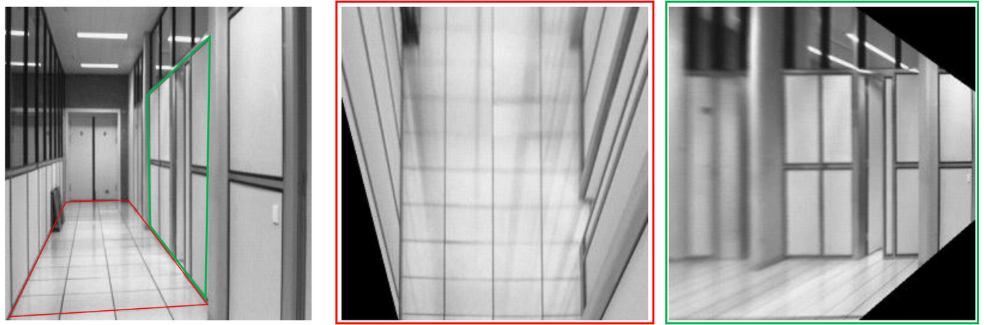
\includegraphics[width=1\textwidth]{./xinhaochuli/2.png}
    \caption{视角旋转得到正对着地板或墙面的图像}
    \label{fig:2}
\end{figure}


如图\ref{fig:2}输入一个这样的走廊图片,我们想要获得视角旋转到正对着地板或墙面的图像。

\begin{enumerate}
  \item 选取输入图像中,平面上的四个点$\{\mathbf{x}_i^{\prime}\}_{i=1}^4$ ,也就是红色梯形的四个角点。
  \item 手动设置输出图像,给出对应的图像坐标系下对应四个点的位置$\{\mathbf{x}_i\}_{i=1}^4$ ,也就是旋转视角后,长方形的四个角点。给定四个点围成的长方形,只要比例和原场景相似即可。例如红色框中的地板,用地板的边长和每个方向的数量可以辅助确定。
  \item 估计单应矩阵$\mathbf{H}$
  \item 将输入图像中,选定的平面上所有的点,warp到手动设置的输出图像中。即直接使用投影变换$\mathbf{x}_i=\mathbf{H}\mathbf{x}_i^{\prime}$
  \item 将$\mathbf{x}_i/\mathbf{x}_i[2]$归一化,然后取出前两维即为对应的图像像素坐标
\end{enumerate}

\subsubsection{数据处理}

数据要求​

​输入​:走廊图像(含明显平面区域,如地板/墙面)。
​标注​:平面区域的4个角点坐标​(源图像梯形顶点 + 目标矩形顶点)。

​采集图像​

使用手机/相机拍摄不同视角的走廊图片(倾斜、俯视、平视)。
确保平面区域(地板)纹理清晰(如瓷砖、木纹),便于角点标注。

​标注点对​

源点:在原图点击梯形4个角点。
目标点:定义矩形角点(如 [(0,0), (w,0), (w,h), (0,h)],保持原比例)。

​存储格式​CSV:
\begin{lstlisting}
  image_path, src_x1, src_y1, dst_x1, dst_y1, src_x2, src_y2, dst_x2, dst_y2, ...
  corridor1.jpg, 56, 65, 0, 0, 368, 52, 300, 0, ...
\end{lstlisting}



\subsubsection{代码构建与结果分析}

\begin{lstlisting}
import cv2
import numpy as np

# 初始化全局变量
points_src = []  # 存储源图像选取点
points_dst = []  # 存储目标位置点
img = None       # 原始图像
img_output = None # 输出图像

def select_points(event, x, y, flags, param):
    """鼠标回调函数:在图像上选取4个点"""
    global points_src, img
    
    if event == cv2.EVENT_LBUTTONDOWN:
        if len(points_src) < 4:
            points_src.append((x, y))
            cv2.circle(img, (x, y), 5, (0, 0, 255), -1)  # 标记红点
            cv2.imshow("Select 4 Points (Source)", img)
            print(f"Selected point {len(points_src)}: ({x}, {y})")
            
            # 选取完4个点后自动计算变换
            if len(points_src) == 4:
                calculate_homography()

def calculate_homography():
    """计算单应性矩阵并执行透视变换"""
    global points_src, points_dst, img, img_output
    
    # 自动计算目标点(基于原始点形成的矩形)
    src_pts = np.array(points_src, dtype=np.float32)
    
    # 计算原始点形成的四边形宽高比
    width = max(np.linalg.norm(src_pts[0]-src_pts[1]), 
               np.linalg.norm(src_pts[2]-src_pts[3]))
    height = max(np.linalg.norm(src_pts[0]-src_pts[3]),
                np.linalg.norm(src_pts[1]-src_pts[2]))
    
    # 创建目标矩形点(保持原始宽高比)
    points_dst = np.array([
        [0, 0],
        [width, 0],
        [width, height],
        [0, height]
    ], dtype=np.float32)
    
    # 计算单应性矩阵 [9,10](@ref)
    H, _ = cv2.findHomography(src_pts, points_dst, cv2.RANSAC, 5.0)
    print(f"\nHomography Matrix:\n{H}")
    
    # 执行透视变换 [9](@ref)
    img_output = cv2.warpPerspective(
        img_original, 
        H, 
        (int(width), int(height)),
        flags=cv2.INTER_LINEAR
    )
    
    # 显示结果
    cv2.imshow("Corrected View", img_output)
    cv2.imwrite("corrected_view.jpg", img_output)
    print("视角校正完成!结果已保存为 corrected_view.jpg")

if __name__ == "__main__":
    # 读取输入图像
    img_path = "corridor.jpg"  # 替换为你的走廊图像路径
    img_original = cv2.imread(img_path)
    if img_original is None:
        print("错误:无法读取图像,请检查路径")
        exit()
    
    img = img_original.copy()
    
    # 创建窗口并设置回调
    cv2.namedWindow("Select 4 Points (Source)")
    cv2.setMouseCallback("Select 4 Points (Source)", select_points)
    
    # 显示操作说明
    print("请在图像上按顺序点击4个点(如地板梯形角点)")
    print("建议顺序:左上→右上→右下→左下")
    
    # 显示图像并等待点选择
    cv2.imshow("Select 4 Points (Source)", img)
    cv2.waitKey(0)
    cv2.destroyAllWindows()
\end{lstlisting}


\subsection{拼接共面场景}

\begin{figure}[h]
    \centering
    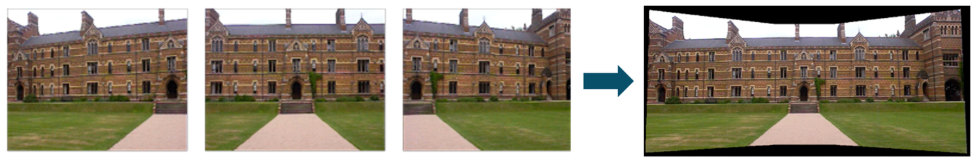
\includegraphics[width=1\textwidth]{./xinhaochuli/3.png}
    \caption{三张不同位置下拍摄的近似共面场景的图像,将它们拼接成全景图}
    \label{fig:3}
\end{figure}

如图\ref{fig:3}输入三张不同位置下拍摄的近似共面场景的图像,将它们拼接成全景图。

\begin{enumerate}
  \item 使用特征提取算法提取输入图像中的特征点,尽量位于建筑物上,并建立匹配关系
  \item 以某一张图像为基准,估计出两个单应矩阵。例如以图像2为基准,估计出$\mathbf{H}_{21}$ 和 $\mathbf{H}_{23}$
  \item 使用单应变换,将点映射到$\mathbf{x}_1^2=\mathbf{H}_{21}\mathbf{x}_1$和$\mathbf{x}_3^2=\mathbf{H}_{23}\mathbf{x}_3$
  \item 对$\mathbf{x}_1^2$和$\mathbf{x}_3^2$执行归一化操作
  \item 应用alpha-blending叠加图像
\end{enumerate}

\subsubsection{数据处理}
\subsubsection{代码构建与结果分析}

\begin{lstlisting}
import cv2
import numpy as np

# 1. 特征提取与匹配
def extract_features_and_match(images):
    """
    提取特征点并建立匹配关系
    :param images: 输入图像列表 [img1, img2, img3]
    :return: 匹配点对字典 {1-2: matches12, 2-3: matches23}
    """
    # 初始化 SIFT 特征检测器
    sift = cv2.SIFT_create()
    
    # 存储关键点和描述符
    kps, descs = [], []
    for img in images:
        gray = cv2.cvtColor(img, cv2.COLOR_BGR2GRAY)
        kp, des = sift.detectAndCompute(gray, None)
        kps.append(kp)
        descs.append(des)
    
    # 使用 FLANN 匹配器
    FLANN_INDEX_KDTREE = 1
    index_params = dict(algorithm=FLANN_INDEX_KDTREE, trees=5)
    search_params = dict(checks=50)
    flann = cv2.FlannBasedMatcher(index_params, search_params)
    
    # 图像1-2匹配
    matches12 = flann.knnMatch(descs[0], descs[1], k=2)
    # 图像2-3匹配
    matches23 = flann.knnMatch(descs[2], descs[1], k=2)
    
    # 应用 Lowe's 比率测试筛选良好匹配
    good_matches12 = []
    for m, n in matches12:
        if m.distance < 0.7 * n.distance:
            good_matches12.append(m)
    
    good_matches23 = []
    for m, n in matches23:
        if m.distance < 0.7 * n.distance:
            good_matches23.append(m)
    
    return {
        '1-2': (kps[0], kps[1], good_matches12),
        '2-3': (kps[2], kps[1], good_matches23)
    }

# 2. 估计单应矩阵
def estimate_homographies(matches_data):
    """
    估计单应矩阵 H21 和 H23
    :param matches_data: 匹配点对数据
    :return: 单应矩阵 H21, H23
    """
    # 提取图像1-2的匹配点
    kp1, kp2, matches12 = matches_data['1-2']
    src_pts12 = np.float32([kp1[m.queryIdx].pt for m in matches12]).reshape(-1, 1, 2)
    dst_pts12 = np.float32([kp2[m.trainIdx].pt for m in matches12]).reshape(-1, 1, 2)
    
    # 计算 H21 (从图像1到图像2)
    H21, mask21 = cv2.findHomography(src_pts12, dst_pts12, cv2.RANSAC, 5.0)
    
    # 提取图像2-3的匹配点
    kp3, kp2, matches23 = matches_data['2-3']
    src_pts23 = np.float32([kp3[m.queryIdx].pt for m in matches23]).reshape(-1, 1, 2)
    dst_pts23 = np.float32([kp2[m.trainIdx].pt for m in matches23]).reshape(-1, 1, 2)
    
    # 计算 H23 (从图像3到图像2)
    H23, mask23 = cv2.findHomography(src_pts23, dst_pts23, cv2.RANSAC, 5.0)
    
    return H21, H23

# 3. 点映射和4. 归一化
def transform_and_normalize_points(H, points):
    """
    应用单应变换并归一化坐标
    :param H: 单应矩阵
    :param points: 输入点集 (N, 2)
    :return: 变换并归一化后的点集 (N, 2)
    """
    # 转换为齐次坐标 (添加第三维1)
    homogeneous_pts = np.hstack((points, np.ones((points.shape[0], 1))))
    
    # 应用单应变换
    transformed_pts = np.dot(H, homogeneous_pts.T).T
    
    # 归一化 (除以第三维)
    normalized_pts = transformed_pts[:, :2] / transformed_pts[:, 2].reshape(-1, 1)
    
    return normalized_pts

# 5. Alpha-blending 图像融合
def alpha_blending(img1, img2, img3, H21, H23):
    """
    应用单应变换并进行alpha-blending图像融合
    :param img1: 图像1
    :param img2: 基准图像2
    :param img3: 图像3
    :param H21: 图像1到图像2的单应矩阵
    :param H23: 图像3到图像2的单应矩阵
    :return: 融合后的全景图像
    """
    # 计算输出图像尺寸
    h2, w2 = img2.shape[:2]
    
    # 变换图像1到图像2的坐标系
    warped1 = cv2.warpPerspective(img1, H21, (w2, h2))
    
    # 变换图像3到图像2的坐标系
    warped3 = cv2.warpPerspective(img3, H23, (w2, h2))
    
    # 创建融合掩码
    mask1 = np.ones_like(warped1, dtype=np.float32)
    mask2 = np.ones_like(img2, dtype=np.float32)
    mask3 = np.ones_like(warped3, dtype=np.float32)
    
    # 应用alpha-blending
    # 重叠区域使用渐变权重
    blended = np.zeros_like(img2, dtype=np.float32)
    
    # 计算权重图
    alpha_map = np.zeros((h2, w2), dtype=np.float32)
    
    # 图像1的权重:左侧权重高,右侧权重低
    for col in range(w2):
        weight = 1.0 - min(col / (w2 / 2), 1.0)
        alpha_map[:, col] = weight
    
    # 图像3的权重:右侧权重高,左侧权重低
    for col in range(w2):
        weight = min(col / (w2 / 2), 1.0)
        alpha_map[:, col] = max(alpha_map[:, col], weight)
    
    # 基准图像2保持中间权重
    alpha_map[:, w2//4:3*w2//4] = 0.5
    
    # 扩展alpha_map到三通道
    alpha_map = cv2.merge([alpha_map, alpha_map, alpha_map])
    
    # 应用融合
    blended = warped1 * (1 - alpha_map) + img2 * alpha_map
    blended = blended * (1 - alpha_map) + warped3 * alpha_map
    
    # 转换为8位图像
    blended = np.clip(blended, 0, 255).astype(np.uint8)
    
    return blended

# 主函数
def main():
    # 读取三张输入图像
    img1 = cv2.imread('building1.jpg')
    img2 = cv2.imread('building2.jpg')  # 基准图像
    img3 = cv2.imread('building3.jpg')
    
    if img1 is None or img2 is None or img3 is None:
        print("错误:无法读取图像文件")
        return
    
    # 1. 特征提取与匹配
    matches_data = extract_features_and_match([img1, img2, img3])
    
    # 2. 估计单应矩阵
    H21, H23 = estimate_homographies(matches_data)
    print(f"H21 矩阵:\n{H21}")
    print(f"H23 矩阵:\n{H23}")
    
    # 3. & 4. 点映射和归一化(示例)
    # 提取图像1的特征点
    kp1, _, matches12 = matches_data['1-2']
    sample_points = np.float32([kp1[m.queryIdx].pt for m in matches12[:5]])
    print("原始点 (图像1):\n", sample_points)
    
    # 变换并归一化
    transformed_points = transform_and_normalize_points(H21, sample_points)
    print("变换并归一化后的点 (图像2坐标系):\n", transformed_points)
    
    # 5. 应用alpha-blending拼接图像
    panorama = alpha_blending(img1, img2, img3, H21, H23)
    
    # 显示并保存结果
    cv2.imshow('Building Panorama', panorama)
    cv2.imwrite('building_panorama.jpg', panorama)
    cv2.waitKey(0)
    cv2.destroyAllWindows()

if __name__ == "__main__":
    main()
\end{lstlisting}

\subsection{由单应矩阵估计纯旋转运动}

在推导平面单应性时,我们引入了$\mathbf{X}_2=\mathbf{R}\mathbf{X}_1+\mathbf{t}$,以及点在平面上从而获得平面约束。

现在考虑一个特例。相机没有平移运动,而仅包含旋转。此时$\mathbf{X}_2=\mathbf{R}\mathbf{X}_1$ 。

这里会发现个神奇的事情,我们不需要引入平面约束就能得到单应性的的约束$\mathbf{x}_2\sim\mathbf{H}\mathbf{x}_1$

这种纯旋转场景下就不用要求匹配点都在平面上了。

假设我们根据图像匹配点,利用单应矩阵估计恢复出$\mathbf{y}_2\sim\mathbf{KHK}^{-1}\mathbf{y}_1$中的$\mathbf{H}$矩阵,这个矩阵$\mathbf{H}$实际上就对应着旋转$\mathbf{R}$ 。而旋转矩阵$\mathbf{R}\in\mathcal{SO}(3)$,因此再对估计出的$\mathbf{H}$矩阵做一下$\mathcal{SO}(3)$的投影,即可得到最终的旋转矩阵估计。




\section{总结与展望}

单应性作为连接2D-3D几何的桥梁,在文物数字化中需突破传统共面假设。未来研究应聚焦鲁棒估计、非平面扩展及深度学习融合,同时结合多模态数据提升重建精度。


  
% 尾页标签, 用于标记页数
\label{EndBody}        


%%%%%%%%%%%%%  参考文献 %%%%%%%%%%%%
\newpage
\pagestyle{empty}

\bibliographystyle{gbt7714-numerical}
\bibliography{xinhaochuli.bib}


%%%%%%%%%%%%% 文档结束 %%%%%%%%%%%%
\end{document}